%
% Main document
% ===========================================================================
% This is part of the document "Project documentation template".
% Authors: brd3, kaa1
%

%---------------------------------------------------------------------------
\documentclass[
	a4paper,					% paper format
	10pt,							% fontsize
	twoside,					% double-sided
	openright,				% begin new chapter on right side
	notitlepage,			% use no standard title page
	parskip=half,			% set paragraph skip to half of a line
]{scrreprt}					% KOMA-script report
%---------------------------------------------------------------------------

\raggedbottom
\KOMAoptions{cleardoublepage=plain}			% Add header and footer on blank pages


% Load Standard Packages:
%---------------------------------------------------------------------------
\usepackage[standard-baselineskips]{cmbright}

\usepackage[ngerman,english]{babel}										% english hyphenation
%\usepackage[latin1]{inputenc}  							% Unix/Linux - load extended character set (ISO 8859-1)
\usepackage[ansinew]{inputenc}  							% Windows - load extended character set (ISO 8859-1)
\usepackage[T1]{fontenc}											% hyphenation of words with �,� and �
\usepackage{textcomp}													% additional symbols
\usepackage{ae}																% better resolution of Type1-Fonts 
\usepackage{fancyhdr}													% simple manipulation of header and footer 
\usepackage{etoolbox}													% color manipulation of header and footer
\usepackage{graphicx}                      		% integration of images
\usepackage{float}														% floating objects
\usepackage{caption}													% for captions of figures and tables
\usepackage{booktabs}													% package for nicer tables
\usepackage{tocvsec2}
\usepackage{hhline}	
\usepackage{multirow}	
\usepackage{pbox}
\usepackage{makecell}
\usepackage{caption}
\usepackage{subcaption}											% provides means of controlling the sectional numbering
%---------------------------------------------------------------------------

% Load Math Packages
%---------------------------------------------------------------------------
\usepackage{amsmath}                    	   	% various features to facilitate writing math formulas
\usepackage{amsthm}                       	 	% enhanced version of latex's newtheorem
\usepackage{amsfonts}                      		% set of miscellaneous TeX fonts that augment the standard CM
\usepackage{amssymb}													% mathematical special characters
\usepackage{exscale}													% mathematical size corresponds to textsize

%---------------------------------------------------------------------------

% Package to facilitate placement of boxes at absolute positions
%---------------------------------------------------------------------------
\usepackage[absolute]{textpos}
\setlength{\TPHorizModule}{1mm}
\setlength{\TPVertModule}{1mm}
%---------------------------------------------------------------------------					
\renewcommand\theadalign{cb}
\renewcommand\theadfont{\bfseries}
\renewcommand\theadgape{\Gape[4pt]}
\renewcommand\cellgape{\Gape[4pt]}		
% Definition of Colors
%---------------------------------------------------------------------------
\RequirePackage{color}                          % Color (not xcolor!)
\definecolor{linkblue}{rgb}{0,0,0.8}            % Standard
\definecolor{darkblue}{rgb}{0,0.08,0.45}        % Dark blue
\definecolor{bfhgrey}{rgb}{0.41,0.49,0.57}      % BFH grey
%\definecolor{linkcolor}{rgb}{0,0,0.8}     			% Blue for the web- and cd-version!
\definecolor{linkcolor}{rgb}{0,0,0}        			% Black for the print-version!
%---------------------------------------------------------------------------

% Hyperref Package (Create links in a pdf)
%---------------------------------------------------------------------------
\usepackage[
	pdftex,ngerman,bookmarks,plainpages=false,pdfpagelabels,
	backref = {false},										% No index backreference
	colorlinks = {true},                  % Color links in a PDF
	hypertexnames = {true},               % no failures "same page(i)"
	bookmarksopen = {true},               % opens the bar on the left side
	bookmarksopenlevel = {0},             % depth of opened bookmarks
	pdftitle = {Template f�r Bachelor Thesis},	   	% PDF-property
	pdfauthor = {brd3},        					  % PDF-property
	pdfsubject = {LaTeX Template},        % PDF-property
	linkcolor = {linkcolor},              % Color of Links
	citecolor = {linkcolor},              % Color of Cite-Links
	urlcolor = {linkcolor},               % Color of URLs
]{hyperref}
%---------------------------------------------------------------------------

% Set up page dimension
%---------------------------------------------------------------------------
\usepackage{geometry}
\geometry{
	a4paper,
	left=28mm,
	right=15mm,
	top=30mm,
	headheight=20mm,
	headsep=10mm,
	textheight=242mm,
	footskip=15mm
}
%---------------------------------------------------------------------------

% Makeindex Package
%---------------------------------------------------------------------------
\usepackage{makeidx}                         		% To produce index
\makeindex                                    	% Index-Initialisation
%---------------------------------------------------------------------------

% Glossary Package
%---------------------------------------------------------------------------
% the glossaries package uses makeindex
% if you use TeXnicCenter do the following steps:
%  - Goto "Ausgabeprofile definieren" (ctrl + F7)
%  - Select the profile "LaTeX => PDF"
%  - Add in register "Nachbearbeitung" a new "Postprozessoren" point named Glossar
%  - Select makeindex.exe in the field "Anwendung" ( ..\MiKTeX x.x\miktex\bin\makeindex.exe )
%  - Add this [ -s "%tm.ist" -t "%tm.glg" -o "%tm.gls" "%tm.glo" ] in the field "Argumente"
%
% for futher informations go to http://ewus.de/tipp-1029.html
%---------------------------------------------------------------------------
\usepackage[nonumberlist]{glossaries}
\makeglossaries
\newglossaryentry{BibTeX}{name={BibTeX},description={Program for the creation of 	bibliographical references and directories in \TeX or \LaTeX documents}}
\newglossaryentry{Index}{name={Index},description={Index with keywords from text}}
\newglossaryentry{LED}{name={LED},description={Light Emitting Diode}}
\newglossaryentry{FPGA}{name={FPGA},description={Field-Programmable Gate Array, integrated circuit that can be reconfigured after manufacturing}}
\newglossaryentry{ARM}{name={ARM},description={Advanced \gls{RISC} Machine, family of \gls{RISC} architectures for computer processors}}
\newglossaryentry{RISC}{name={RISC},description={Reduced Instruction Set Computing, a \gls{CPU} design strategy}}
\newglossaryentry{CPU}{name={CPU},description={Central Processing Unit, an important part of a computer}}
\newglossaryentry{API}{name={API},description={Application Programming Interface}}
\newglossaryentry{JSON}{name={JSON},description={JavaScript Object Notation, data-interchange format}}
\newglossaryentry{atan2}{name={atan2},description={arctangent function with two arguments}}
\newglossaryentry{VGA}{name={VGA},description={Video Graphics Array, resolution of 640x480}}
\newglossaryentry{QVGA}{name={QVGA},description={Quarter Video Graphics Array, resolution of 320x240}}
\newglossaryentry{UVGA}{name={UVGA},description={Ultra Video Graphics Array, resolution of 1280x960}}
\newglossaryentry{IP}{name={IP},description={Intellectual Property}}




%---------------------------------------------------------------------------

% Intro:
%---------------------------------------------------------------------------
\begin{document}                              	% Start Document
\settocdepth{section}														% Set depth of toc
\pagenumbering{roman}														
%---------------------------------------------------------------------------

\providecommand{\heading}{Title of Thesis}		%  Insert Title of Thesis here					% Titel der Arbeit aus Datei titel.tex lesen
\providecommand{\versionnumber}{1.2}			%  Hier die aktuelle Versionsnummer eingeben
\providecommand{\versiondate}{07.02.2014}		%  Hier das Datum der aktuellen Version eingeben				% Versionsnummer und -datum aus Datei version.tex lesen

% Set up header and footer
%---------------------------------------------------------------------------
\makeatletter
\patchcmd{\@fancyhead}{\rlap}{\color{bfhgrey}\rlap}{}{}		% new color of header
\patchcmd{\@fancyfoot}{\rlap}{\color{bfhgrey}\rlap}{}{}		% new color of footer
\makeatother

\fancyhf{}																		% clean all fields
\fancypagestyle{plain}{												% new definition of plain style	
	\fancyfoot[OR,EL]{\footnotesize \thepage} 	% footer right part --> page number
	\fancyfoot[OL,ER]{\footnotesize \heading, Version \versionnumber, \versiondate}	% footer even page left part 
}

\renewcommand{\chaptermark}[1]{\markboth{\thechapter.  #1}{}}
\renewcommand{\headrulewidth}{0pt}				% no header stripline
\renewcommand{\footrulewidth}{0pt} 				% no bottom stripline

\pagestyle{plain}
%---------------------------------------------------------------------------


% Title Page and Abstract
%---------------------------------------------------------------------------
%%
% Project documentation template
% ===========================================================================
% This is part of the document "Project documentation template".
% Authors: brd3, kaa1
%

\begin{titlepage}


% BFH-Logo absolute placed at (28,12) on A4 and picture (16:9 or 15cm x 8.5cm)
% Actually not a realy satisfactory solution but working.
%---------------------------------------------------------------------------
\setlength{\unitlength}{1mm}
\begin{textblock}{20}[0,0](28,12)
	
\includegraphics[scale=1.0]{images/BFH_Logo_B.png}
\end{textblock}

% Institution / titel / subtitel / authors / experts:
%---------------------------------------------------------------------------
\begin{flushleft}

\vspace*{21mm}

\fontsize{26pt}{40pt}\selectfont 
\heading				\\							% Read heading from file leader/title.tex
\vspace{2mm}

\fontsize{16pt}{24pt}\selectfont\vspace{0.3em}
Place your subheading here 			\\				% Insert subheading
\vspace{5mm}

\fontsize{10pt}{12pt}\selectfont
\textbf{Description of thesis (semester- / Bachelor thesis / etc.)} \\		% Insert text
\vspace{7mm}

% Abstract (eingeben):
%---------------------------------------------------------------------------
\begin{textblock}{150}(28,100)
\fontsize{10pt}{12pt}\selectfont
[Insert short text (abstract) if desired] \\ 
This document serves as a template for the compilation of reports according to the guidelines of the BFH. The template is written in LATEX and supports the automatic writing of various directories, references, indexing and glossaries. This small text is a summary of this document with a length of 4 to max. 8 lines. \\ 
The cover picture may be turned on or off in the lines 157/158 of the file template.tex.
\end{textblock}

\begin{textblock}{150}(28,225)
\fontsize{10pt}{17pt}\selectfont
\begin{tabbing}
xxxxxxxxxxxxxxx\=xxxxxxxxxxxxxxxxxxxxxxxxxxxxxxxxxxxxxxxxxxxxxxx \kill
Degree course:	\> [z.B. Electrical and Communication Engineering]	\\		% insert name of degree course
Authors:		\> [Test Peter, M\"uster R\"os\"a]		\\					% insert names
Tutor:	\> [Dr.~Xxxx Xxxx, Dr.~Yyyy Yyyy]		\\							% insert names
Constituent:	\> [Wwwww AG]					\\							% insert names
Experts:		\> [Dr.~Zzzz Zzzz]				\\							% insert names
Date:			\> \versiondate					\\							% read from file leader/version.tex
\end{tabbing}

\end{textblock}
\end{flushleft}

\begin{textblock}{150}(28,280)
\noindent 
\color{bfhgrey}\fontsize{9pt}{10pt}\selectfont
Berner Fachhochschule | Haute \'ecole sp\'ecialis\'ee bernoise | Bern University of Applied Sciences
\color{black}\selectfont
\end{textblock}


\end{titlepage}

%
% ===========================================================================
% EOF
%
		% activate for frontpage without picture
%
% Project documentation template
% ===========================================================================
% This is part of the document "Project documentation template".
% Authors: brd3, kaa1
%

\begin{titlepage}


% BFH-Logo absolute placed at (28,12) on A4 and picture (16:9 or 15cm x 8.5cm)
% Actually not a realy satisfactory solution but working.
%---------------------------------------------------------------------------
\setlength{\unitlength}{1mm}
\begin{textblock}{20}[0,0](28,12)
	
\includegraphics[scale=1.0]{images/BFH_Logo_B.png}
\end{textblock}

\begin{textblock}{154}(28,48)
	\begin{picture}(150,2)
		\put(0,0){\color{bfhgrey}\rule{150mm}{2mm}}
	\end{picture}
\end{textblock}

\begin{textblock}{154}[0,0](28,50)
	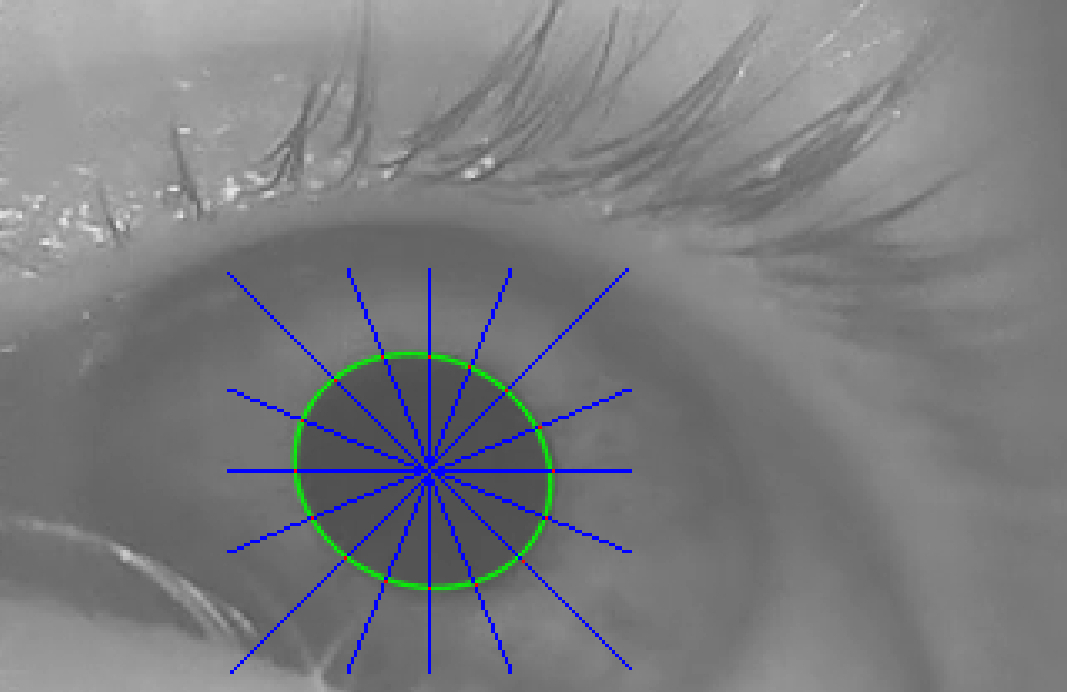
\includegraphics[width=0.974\linewidth]{images/good_fit.png}			% define cover picture
\end{textblock}

\begin{textblock}{154}(28,147)
	\begin{picture}(150,2)
		\put(0,0){\color{bfhgrey}\rule{150mm}{2mm}}
	\end{picture}
\end{textblock}
\color{black}

% Institution / titel / subtitel / authors / experts:
%---------------------------------------------------------------------------
\begin{flushleft}

\vspace*{125mm}

\fontsize{26pt}{28pt}\selectfont 
\heading				\\							% Read heading from file leader/title.tex
\vspace{2mm}

\fontsize{16pt}{20pt}\selectfont\vspace{0.3em}
Bachelor Thesis			\\				% Insert subheading
\vspace{5mm}

\fontsize{10pt}{12pt}\selectfont
\textbf{} \\		% Insert text
\vspace{3mm}

% Abstract (eingeben):
%---------------------------------------------------------------------------
\begin{textblock}{150}(28,190)

\end{textblock}

\begin{textblock}{150}(28,225)
\fontsize{10pt}{17pt}\selectfont
\begin{tabbing}
xxxxxxxxxxxxxxx\=xxxxxxxxxxxxxxxxxxxxxxxxxxxxxxxxxxxxxxxxxxxxxxx \kill
Degree course:	\> Electrical and Communication Engineering	\\		% insert name of degree course
Author:		\> Timoth\a'{e}e Mollet		\\					% insert names
Tutor:	\> Prof. Dr. Theo Kluter		\\							% insert names					\\							% insert names
Expert:		\> Felix Kunz				\\							% insert names
Date:			\> \versiondate					\\							% read from file leader/version.tex
\end{tabbing}

\end{textblock}
\end{flushleft}

\begin{textblock}{150}(28,280)
\noindent 
\color{bfhgrey}\fontsize{9pt}{10pt}\selectfont
Berner Fachhochschule | Haute \'ecole sp\'ecialis\'ee bernoise | Bern University of Applied Sciences
\color{black}\selectfont
\end{textblock}


\end{titlepage}

%
% ===========================================================================
% EOF
%
		% activate for frontpage with picture
% Control of versions :
% -----------------------------------------------

\begin{textblock}{180}(15,150)
\color{black}
\begin{huge}
Versions
\end{huge}
\vspace{10mm}

\fontsize{10pt}{18pt}\selectfont
\begin{tabbing}
xxxxxxxxxxx\=xxxxxxxxxxxxxxx\=xxxxxxxxxxxxxx\=xxxxxxxxxxxxxxxxxxxxxxxxxxxxxxxxxxxxxxxxxxxxxxx \kill
Version	\> Date	\> Status			\> Remarks		\\
0.1	\> 01.08.2013	\> Draft		\> Lorem ipsum dolor sit amet	\\	
0.2	\> 21.08.2013	\> Draft		\> Phasellus scelerisque	\\ 
0.3	\> 02.09.2013	\> Draft		\> Donec eget aliquam urna. Lorem ipsum dolor sit amet	\\ 
1.0	\> 26.01.2014	\> Final		\> Lorem ipsum dolor sit ametPhasellus scelerisque, leo sed iaculis ornare 	\\ 
1.1	\> 31.01.2014	\> Correction	\> Layout changed	\\
1.2	\> 07.02.2014	\> Addition		\> Chapter 1.1 extended	\\
\end{tabbing}

\end{textblock}

\cleardoubleemptypage
\setcounter{page}{1}
\cleardoublepage
\phantomsection 
\addcontentsline{toc}{chapter}{Management Summary}
\chapter*{Management Summary}
\label{chap:managementSummary}

Eye-tracking offers important insights about hand-eye-coordination and visual search techniques of an athlete. An eye-tracking system for sports needs a high accuracy, portability and high temporal resolution.

Such a device is under development at the Institute for Human Centered Engineering. The system uses two cameras per eye to capture infrared images. The images should be used to determine the gaze direction of the athlete. An important component for that is the digital recognition of the pupil. This is currently not implemented satisfactory.

Until now, the detection of the pupil was achieved with a hardly tested algorithm. This algorithm should be improved so that it is more stable and accomplish a better accuracy. Additionally, the algorithm needs to run on the portable hardware of the eye-tracking system.

Test data is required to compare the accuracy of the algorithms. This data needs to consist of known actual values. To achieve that, an animated and accurate model of the eye and the eye-tracking system should be created. This model should be flexible so that pictures for different scenarios can be generated. The rotation of the eyes during the animation builds a reference for results.

The algorithm uses the pictures from the model to generate pupil data. A partner work uses the pupil data to calculate a gaze direction. It is now possible to determine measurement uncertainty with the known rotation of the model as reference.
\cleardoubleemptypage
%---------------------------------------------------------------------------

% Table of contents
%---------------------------------------------------------------------------
\tableofcontents
\cleardoublepage
%---------------------------------------------------------------------------

% Main part:
%---------------------------------------------------------------------------
\pagenumbering{arabic}

\chapter{Introduction}
\label{chap:introduction}

This document serves to illustrate the \LaTeX{} template on the basis of the corporate design\index{Corporate Design} of the Bern University of Applied Sciences\index{Bern University of Applied Sciences} as well as a manual for its use. It is assumed that the user already has some experience with \LaTeX{} or is willing to familiarize with the subject. In the bibliography the user finds some useful information on \LaTeX{} on various books and documents on the Internet.

% Eintr�ge im Verzeichnis erscheinen lassen ohne hier eine Referenz einzuf�gen
\nocite{kopka:band1}
\nocite{raichle:bibtex_programmierung}
\nocite{MiKTeX}
\nocite{KOMA}
\nocite{TeXnicCenter}
\nocite{Marti06}
\nocite{Erbsland08}
\nocite{juergens:einfuehrung}
\nocite{juergens:fortgeschritten}

\section{Organising Documents}
\label{sec:einleitung_aufbau}

This document is structured according to the documentation of a project work or a thesis\index{thesis}. In Chapter \ref{chap:instructions}, the packages used are briefly explained, and instructions are given, how the bibliography and the glossary are to be used. Chapter \ref{chap:typeareatest} presents a sample chapter to audit the type area.

In figure \ref{fig:file_structure} the file structure is shown for this template.

\begin{figure}[H]
	\centering
		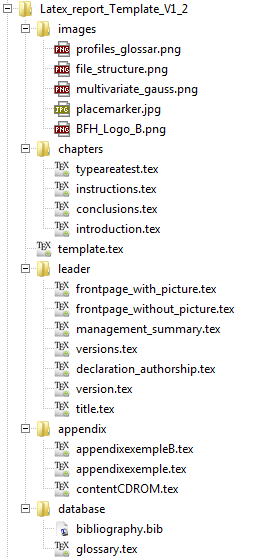
\includegraphics[scale=0.85]{images/file_structure.png}
	\caption{File structure}
	\label{fig:file_structure}
\end{figure}

\section{Contact}
\label{sec:introduction_contact}

The manufacturers of this template welcome any suggestions for improvement. Chapter \ref{sec:introduction_suggestions} shows possible suggestions for improvement\index{suggestions}.

\begin{table}[H]
	\centering
		\begin{tabular}{lll} \toprule
			\textbf{First Name Last Name} & \textbf{E-mail} & \textbf{Function} \\ \midrule
			Alfred Kaufmann & alfred.kaufmann@bfh.ch & Employer, Project Management, \\
			& & Supplements, Improvements \\ \midrule
			Fritz Dellsperger & Retired & Tips on the structure and layout \\ \midrule
			David Burri & Contracted out & First compilation of the Template \\ \bottomrule
		\end{tabular}
	\caption{Contact Persons}
	\label{tab:Contact Persons}
\end{table}


\section{Suggestions for Improvement}
\label{sec:introduction_suggestions}

\begin{itemize}
	\item Create a BFH Style Files
	\item Template for the Compilation of presentations with \LaTeX{}
\end{itemize}



\chapter{Instructions}
\label{chap:instructions}

The following table shows some of the most important packages\index{packages} used in the \LaTeX{} template.

\begin{table}[H]
	\centering
		\begin{tabular}{p{0.13\textwidth} p{0.75\textwidth}} \toprule
			\textbf{Package} & \textbf{Function} \\ \midrule
			\texttt{cmbright}\index{cmbright} & sans serif font "Computer Modern Bright", which supports text encodings\index{text encodings} OT1, T1 and TS1, as well as the mathematical signs and AMS symbols \\ \midrule
			\texttt{ae} & provides better resolution fonts in PDF files \\ \midrule
			\texttt{fancyhdr}\index{fancyhdr} & easy adjustment of head- and foot lines \\ \midrule
			\texttt{graphicx}\index{graphicx} & integration of graphics in \LaTeX{} documents \\ \midrule
			\texttt{booktabs}\index{booktabs} & better presentation of tables \\ \midrule
			\texttt{textpos}\index{textpos} & simplified and absolute positioning of boxes on the page \\ \midrule
			\texttt{hyperref}\index{hyperref} & package to complie links into PDF files \\ \midrule
			\texttt{geometry}\index{geometry} & simplified and improved adaptation of the standard type area \\ \midrule
			\texttt{makeidx}\index{makeidx} & simple Index compilation (see section \ref{sec:instructions_index}) \\ \midrule
			\texttt{glossaries}\index{glossaries} & compilation of glossaries (see section \ref{sec:instructions_glossay}) \\ \bottomrule
		\end{tabular}
	\caption{Packages}
	\label{tab:packages}
\end{table}


\section{Subject Indices}
\label{sec:instructions_index}

\LaTeX{} is not able to create an \gls{Index}\index{Index} in the basic configuration. This can be created in \LaTeX{} with the \texttt{makeidx} package and the \texttt{makeindex}\index{makeindex} program. The following page contains a detailed explanation of how the package works, and its application:

\begin{center}
	\url{http://en.wikibooks.org/wiki/LaTeX/Indexing}
\end{center}

Roughly summarized the following points are needed for an index:

\begin{itemize}
	\item Embed the package \texttt{makeidx}.
	\item Initialize the compilation with the command \texttt{\textbackslash makeindex}.
	\item Continuously initializing words in the text with the command \texttt{\textbackslash index\{\}}.
	\item During the first passage of the document's compilation, the directory is created and definitions marked with \texttt{\textbackslash index\{\}} are stored in the \texttt{.idx} file.
	\item During the second passage the \texttt{.idx} file is sorted, formatted and stored as \texttt{.ind} file whereas \LaTeX{} then inserts the \texttt{.ind} file into the document.
\end{itemize}

\section{Glossay}
\label{sec:instructions_glossay}

A glossary\index{glossary} can also be created in \LaTeX{} with the \texttt{makeindex} program and the \texttt{glossaries} package. The following list shows the procedure to generate a glossary:

\begin{itemize}
	\item Integration of the package \texttt{glossaries}.
	\item If necessary, a personal database may be created including glossary entries. This template works with such a database, which is stored in the \texttt{database}folder. Entries from the database are only written in the directory if the word in the text is actually stated.
	\item With the \texttt{\textbackslash makeglossaries} command a new compilation is initialized.
	\item New entries can be created with the command \\ \texttt{\textbackslash newglossaryentry\{<SHORTCUT>\}\{name=\{<NAME>\},description=\{<DESCRIPTION>\}\}}.
	\item In the text continuously referencing words with the command \texttt{\textbackslash gls\{<SHORTCUT>\}}.
	\item Similar to the compilation of the index, the directory is only embedded into the document  during the second passage.
\end{itemize}

In order to work accurately, the glossary must be compiled with \texttt{makeindex} after post-editing the document. For this the following code in the command line is to be executed:

\begin{center}
	\texttt{makeindex -s template.ist -t template.glg -o template.gls template.glo}
\end{center}

With most \LaTeX editors, this can be stated as a post-processing step. The following explanation is for the TeXnicCenter program. Under the menu "Build" > "Define Output Profile..." (short: alt + F7) in the "Postprocessor" register, the window shown in Figure \ref{fig:postprocessing} can be found. Then it is necessary to insert a new entry, when an application as well as an argument must be specified. The application can be found in the MiKTeX installation (\texttt{..\textbackslash MiKTeX X.X\textbackslash miktex\textbackslash bin\textbackslash makeindex.exe}). As an argument, the following line must be entered:

\begin{center}
	\texttt{-s \string"\%tm.ist\string" -t \string"\%tm.glg\string" -o \string"\%tm.gls\string" \string"\%tm.glo\string" }
\end{center}

\begin{figure}[H]
	\centering
		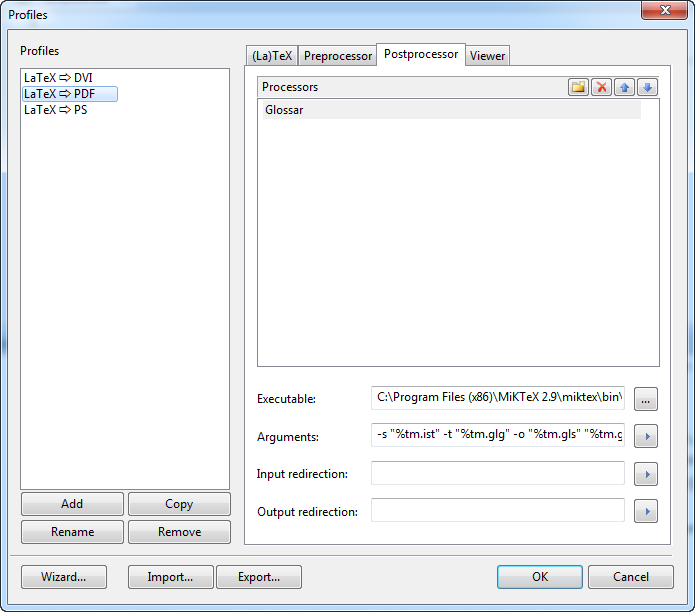
\includegraphics[scale=0.6]{images/profiles_glossar.png}
	\caption{Post-processing}
	\label{fig:postprocessing}
\end{figure}


\section{Bibliography}
\label{sec:instructions_bibliography}

To compile a bibliography\index{bibliography} one must resort to \gls{BibTeX}. The folder \texttt{database} includes a \texttt{.bib} file with various database entries. How the entries are to be compiled, can be taken from various sources of the Internet or books. The entries in the database will only be written to the directory of the document when the source is actually cited in the text.

Under the following addresses further explanations are found in order to compile the database and its use:

\begin{itemize}
	\item \url{http://en.wikipedia.org/wiki/BibTeX}
	\item \url{http://www.bibtex.org/}
\end{itemize}



\chapter{Model}
\label{chap:Model}

A very important step in hardware and software development is testing. For an eye tracking system it requires a big effort to do this with real data. The reason for that is the information where the participant looks at each moment needs to be recorded alongside of the video streams. For this project real time data processing is needed as there is no hardware available on Gazelle Compute to encode or store the video streams of the cameras.

A simple way of generating new data where the gaze direction and the camera positions are known would simplify the process of optimising the algorithm. 
\section{3D-Modeling Software}
\label{sec:whatIsImportant}

The 3D-Modeling software to create the model needs to fulfill a few requirements:
\begin{itemize}
	\item Correct representation of refracting light
	\item Create animations 
	\item \gls{API} that allows scripting
	\begin{itemize}
		\item Set position and rotation of certain objects at a certain frame
		\item Set camera properties and which camera is active
		\item Read the position and rotation of objects at any frame
	\end{itemize}
	\item (optional)Be free
	\item (optional)Run on Linux
	\begin{itemize}
		\item Server that can be used to render runs Linux containers
	\end{itemize}
	\item (optional)Be easy to learn
\end{itemize}

Blender is able to match all requirements although the last one might be debatable. You can apply a material property to a surface. This includes refracting. Rotation and position of objects can be inserted as key frames and it interpolates the steps in-between. 

Blender is also an open source project that is built with Python and has a powerful \gls{API} that gives access to nearly everything.
\section{Requirements for the Model}
In order to create a flexible model that is close to the reality, the model needs to follow the following requirements:
\begin{itemize}
	\item Correctly represent a human eye
	\item Accommodate for different eye parameters
	\begin{itemize}
		\item Eye diameter
		\item Distance between Eyes
	\end{itemize}
	\item Correctly represent camera placement and rotation
	\item Correctly represent camera properties
	\begin{itemize}
		\item Resolution
		\item Frame rate
		\item Field of View
	\end{itemize}
	\item Gaze direction can be animated
	\item Classes rotation and position can be animated
	\item Front facing cameras records gaze direction
\end{itemize}

\section{Human Eye}
A side view of a human eye model is visible in \ref{fig:humanEyeModel}. The camera can only see the front part of the eye. As a result only the cornea, anterior chamber and the iris need to be modelled correctly. The lens can be simplified by a black surface. 

It might be counter intuitive that the cornea extends as much out of the eyeball as visible in \ref{fig:humanEyeModel}. An easy way to verify that is to close the eye and move the eyes while holding a finger on the eyelid.
\label{sec:theHumanEye}
\begin{figure}[H]
	\centering
	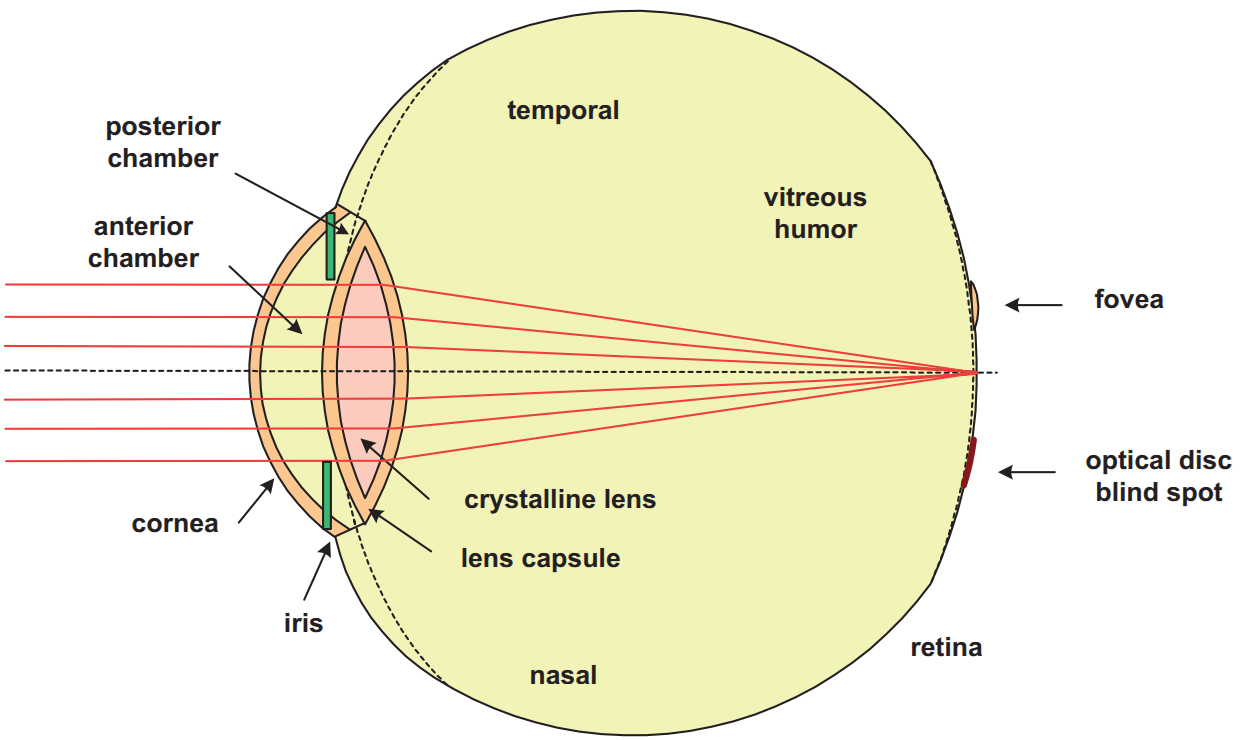
\includegraphics[scale=0.3]{images/human_eye_model.png}
	\caption{Side view of a human eye model \cite{gross:opticalSystems}}
	\label{fig:humanEyeModel}
\end{figure}

There are a few models with different values for the refracting indexes, radii and distances but they vary very little. So the simplified Gullstrand eye was chosen for the model.

\begin{table}[!htb]
\centering
\begin{tabular}{@{}|l|l|l|l|l|l|l|@{}}
	\hline
	\multirow{2}{*}{} & \multicolumn{3}{l|}{\thead{Relaxed}} & \multicolumn{3}{l|}{\thead{Accomodated}} \\ \hhline{~------}
	\thead{ Notaton\\{}} &  \thead{Radius r \\ {}[mm] }        & \thead{Thickness d\\ {}[mm]}    & \thead{Index n\\ {}}        & \thead{Radius r \\ {}[mm] }& \thead{Thickness d \\ {}[mm] }& \thead{Index n\\{} }    \\ \hline
	cornea     &  7.70        & 0.50      & 1.376       &  7.70   &0.50  & 1.376\\ \hline
	anterior chamber & 6.80        & 3.10     & 1.336       & 6.80    & 2.70&1.336 \\ \hline
	crystalline lens     &  10.0    & 3.60          & 1.4085    & 5.33   &   4.0  &  1.426 \\ \hline
	vitreous humor    p  & -6.00      & 17.187         & 1.336    & -5.33  & 13.816  &  1.336  \\ \hline
\end{tabular}
\caption{Properties of the eye with the simplified Gullstrand eye. \cite{gross:opticalSystems}}
\label{tab:gullstrandEye}
\end{table}

A human eye has on average a diameter of 24mm and the distance between the eyes ranges from 56mm to 72mm with the mean for men at 65mm and 62.6mm for women. \cite{gross:opticalSystems}
\section{Base Model}
\label{sec:theModel}

While there are quite a few parameters that need to be adjusted, some will remain the same. This can be incorporated into a base model that can then be adjusted by a script for each render.

This base model is centred around an accurate eye model that is built with the properties mentioned in section \ref{sec:theHumanEye}. Every eye is a group that can be manipulated with a script as one object. This includes a directed light cone that points where the eye is looking.

An existing model of the glasses is used and placed to approximately represent the position on a human head. Cameras are placed into the their cutouts in the glasses. The rotation is approximated to capture an average positioned eye correctly. The light cones that represent the gaze direction illuminate a small portion of a wall, which is captured by the front facing camera and is visible in figure \ref{fig:base3D}. Similar to the eye, the cameras and the glasses build a single object that can be moved and rotated. The result can be seen in figure \ref{fig:baseModel}
\begin{figure}
	\begin{subfigure}{.5\textwidth}
		\centering
		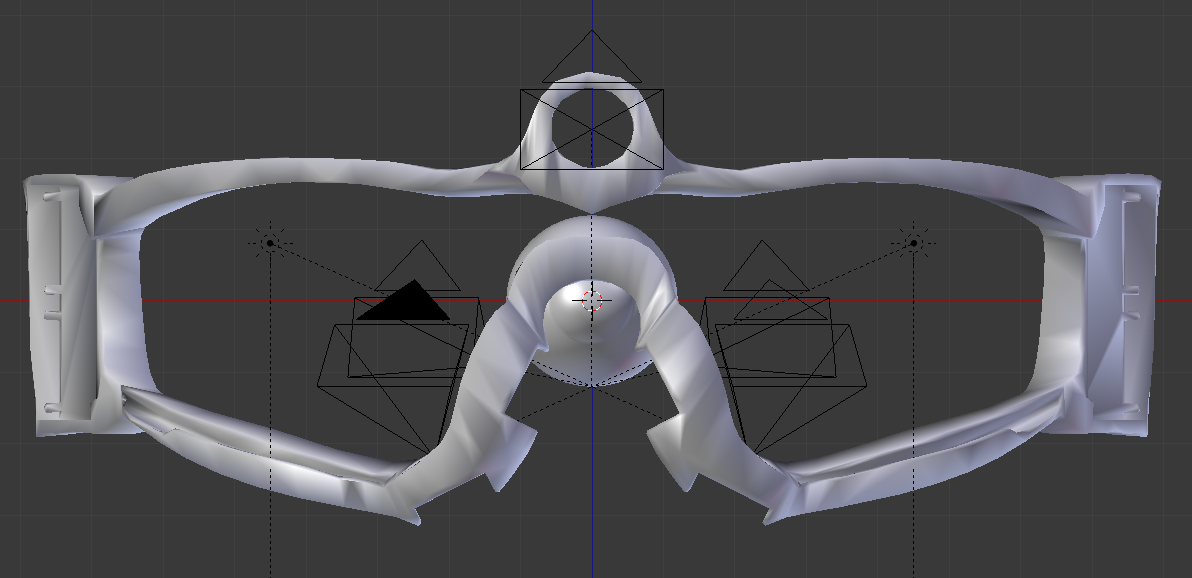
\includegraphics[width=0.9\linewidth]{images/base_model_front.png}
		\caption{Front view of base model}
		\label{fig:baseFront}
	\end{subfigure}
	\begin{subfigure}{.5\textwidth}
		\centering
		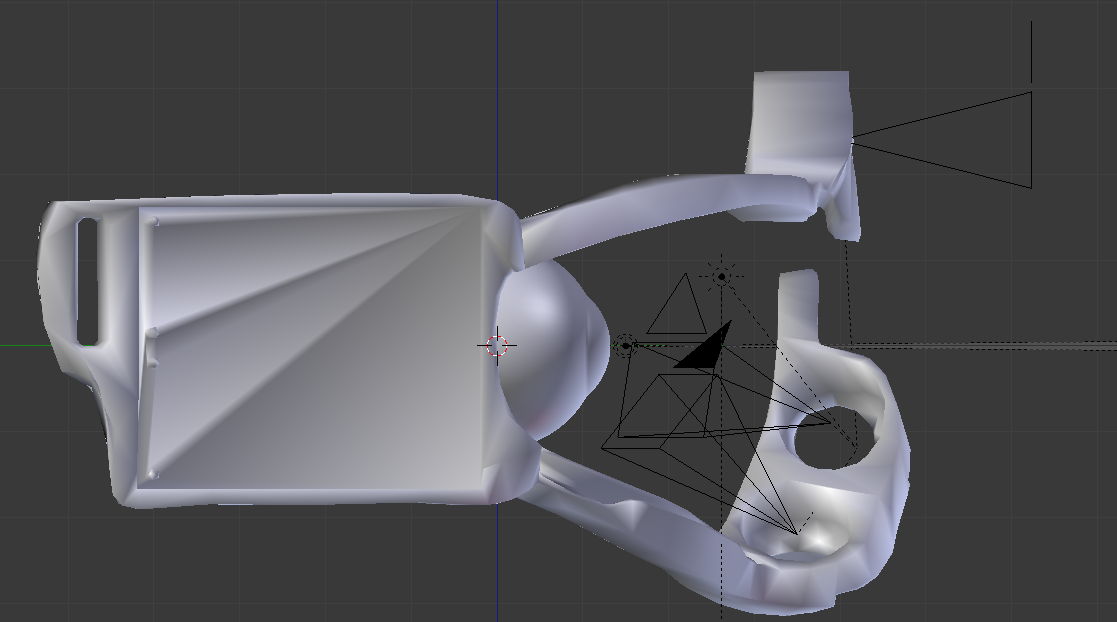
\includegraphics[width=0.787\linewidth]{images/base_model_side.png}
		\caption{Side view of base model}
		\label{fig:baseSide}
	\end{subfigure}
	\begin{subfigure}{.5\textwidth}
		\centering
		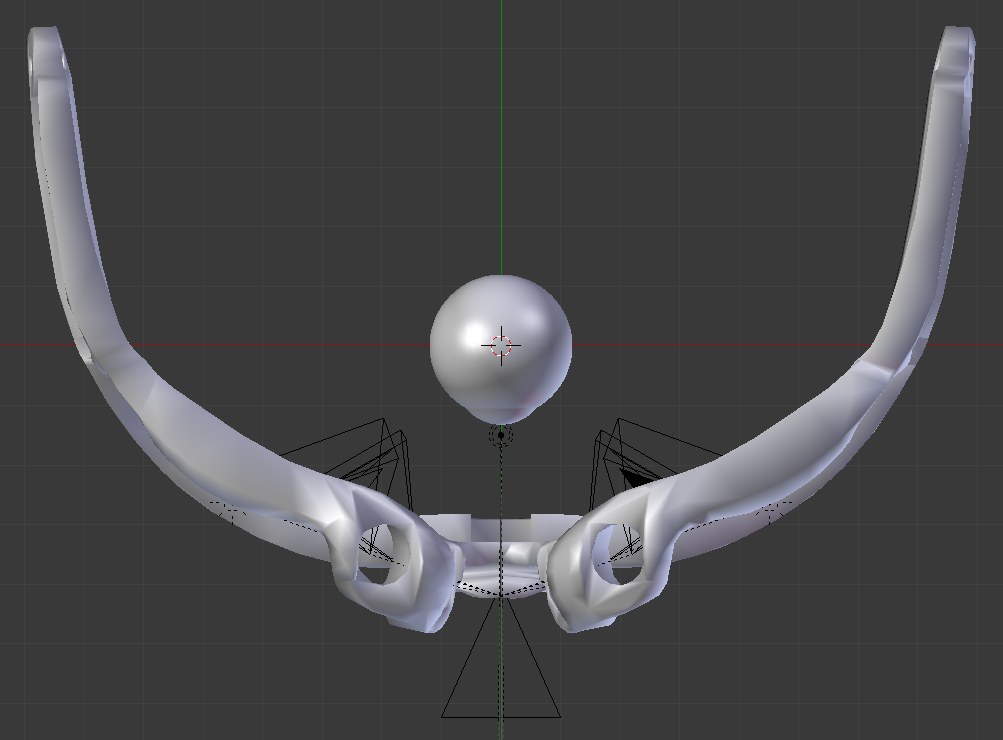
\includegraphics[width=0.9\linewidth]{images/base_model_bottom.png}
		\caption{Bottom view of base model}
		\label{fig:baseBottom}
	\end{subfigure}
	\begin{subfigure}{.5\textwidth}
		\centering
		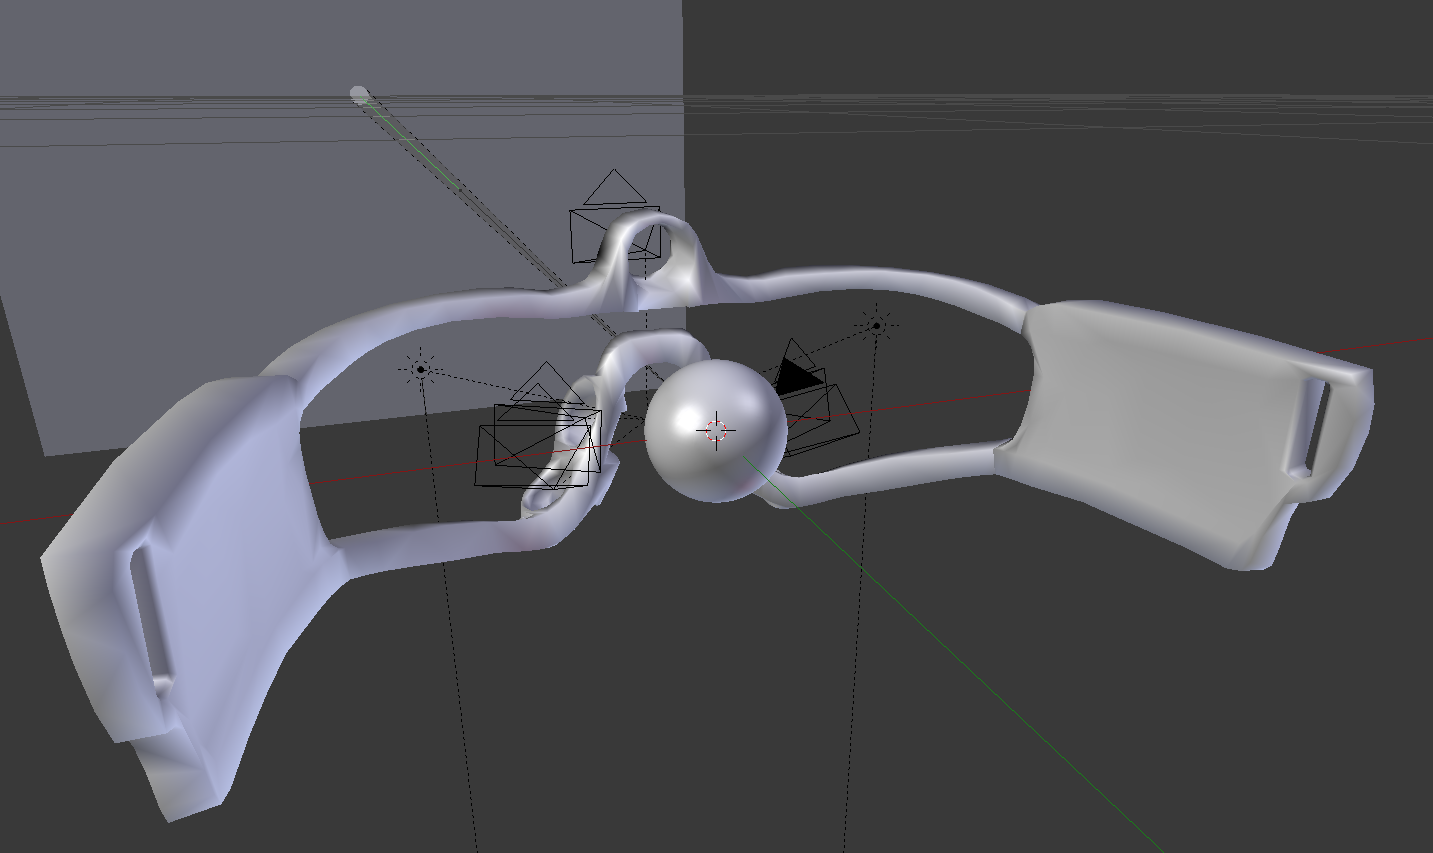
\includegraphics[width=0.9\linewidth]{images/base_model_3D.png}
		\caption{3D-view of base model that shows also the light cone that follows the eye rotation}
		\label{fig:base3D}
	\end{subfigure}
	\caption{Finished base model with eyes in the center. A Script will place the eye correctly and generate an animation from the model that is shown here.}
	\label{fig:baseModel}
\end{figure}
\section{Scripting}
The base model alone is not enough to create meaningful results. Because there is no animation, the eyes are not placed and Blender would just render one camera. Additionally, the position and rotation of the eye and glasses needs to be logged for every frame. Otherwise, they can't be compared with the final gaze direction results. A simple way of configuring the script is needed to allow a wide variety of animations to be created.
\subsubsection{Automate Animation}
The script is written in Python because Blender offers a powerful Python \gls{API} that allows a script to modify every property in a model.
\gls{JSON} is a simple data-interchange format that is easy to read and write for humans. Sites such as \url{http://jsoneditoronline.org/} offer a convenient way to modify \gls{JSON}. The script uses a \gls{JSON} file with all the properties as input. It adjusts the values in the model and saves a modified blend file for each camera. This blend file is ready to be rendered without any further modification. The properties include static parameters such as the eye position and diameter. But also dynamic information for key frames such as the rotation of the eye and position of the glasses.
\subsubsection{Automate Process}
Even with the script, the process to generate render output is still very time consuming. First the script needs to be applied to base model, which produces the blend files that are ready to render. For each file a render job needs to be started. 

A Makefile offers a convenient way to automate the stages further. Additionally, it makes it simple to clean the whole mess up once the generated or rendered files are not needed anymore. 
With the Makefile the whole process is shorter and easier to remember:
\textbf{}
\begin{lstlisting}
#export config file
export ANIMATION_JSON=animation.json
make
make render
\end{lstlisting}

After a few hours test data is ready to be used for analysis.




\chapter{Pupil Detection}
\label{chap:pupildetection}
 Without test data it is very hard to improve an algorithm. The generated pictures of the last chapter lay the groundwork to detect the pupil digitally.
 
 This chapter shows how the current algorithm tries to detect a pupil. Improvements are presented that achieve a better result. 
\section{Overview of Existing Algorithm}
The general sequence of the algorithm can be described as follows:
\begin{enumerate}
	\item Find darkest spot
	\item Extract rays  starting from the darkest spot from the image
	\item Transit the rays with a filter of certain length to detect edges
	\item Fit an ellipse on the detected edges with the least square method
\end{enumerate}
The darkest spot is determined by a raster with a fixed distance between points. For each point the average with the surrounding eights point is calculated. The point with the darkest average is the startpoint for the rest of the algorithm.

Outgoing from the startpoint rays are stamped out by the starburst IP that is described in "Eye Tracking for Sports, Chapter 18.5" 

The difference to the next pixel is calculated for each ray that is stamped out by the starburst IP. Because the edge may not lie on a single pixel, surrounding differences are added together to build a score for each pixel. This score is positive for transitions from a darker pixel to a brighter. The pixel with the highest score is determined as detected edge. So only edges that transit from dark to bright can be detected.

Every edgepoint is handed over to a weighted least square method to find a ellipse that fits all the points well. The residuals of the lest square fitting are used to calculate how well the ellipse fits on the points.
\subsubsection{Testing}
The algorithm was tested with pictures that were inserted at compile time with the parameters of the ellipse as output. The result was then compared with the result. This is not efficient and is addressed in the next section.
\section{Improve Testing}
\label{sec:improveTesting}
It is very time consuming to generate picture data that can be compiled and to compare the output of the program with what is expected. A better way is when a tool can read a video file and display the result of the algorithm visually on each picture. 

The program "Gazelle View" that was developed during the project study can already open and play video files. Because of the modular design of Gazelle View it is simple to insert the algorithm during the decode phase and paint the rays, the detected edges and the fitted ellipse on the image.

All data that was produced by the algorithm may also hold important information to find bugs or problems with the algorithm. In order to display that data besides the frame all data is packed into a struct and displayed in a Treeview beside the frame. 

The next step to improve testing would be to automate it and ideally condense the performance of the algorithm to parameters such as the mean and variance of the accuracy.

This should be done on a wide variety of test data, at best with high frame rate pictures that were captured with the eye tracking system. For each of those pictures an ellipse has to be fitted manually and stored as a golden reference. As this needs to be done for a lot of pictures the process of generating the reference needs to be simplified.
\section{Outliers}
The supplied algorithm does not differentiate between edges that are from the pupil or other edges from hair or the eyelid. The algorithm works fine when every edge is a right one as seen in figure \ref{fig:oldGood}. But as a consequence to the least square method a single false detection severely alters the fitted ellipse as it happens in figure \ref{fig:oldOutlier}. 
\begin{figure}
	\begin{subfigure}{.5\textwidth}
		\centering
		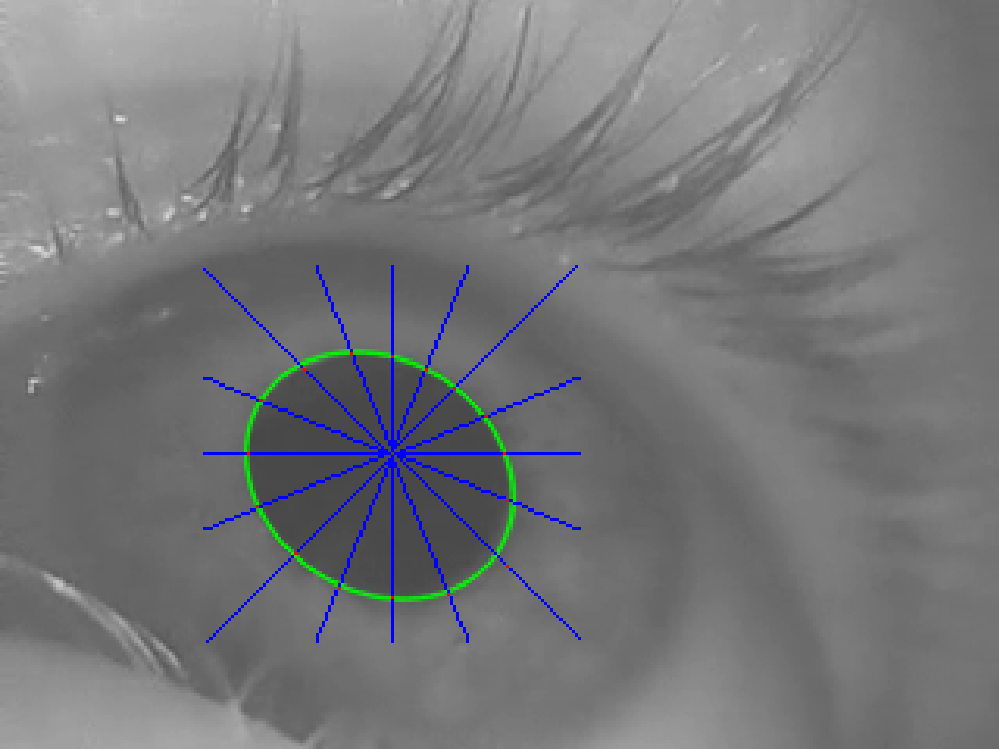
\includegraphics[width=\linewidth]{images/good_fit_old.png}
		\caption{Fitting of Ellipse without outliers}
		\label{fig:oldGood}
	\end{subfigure}%
	\begin{subfigure}{.5\textwidth}
		\centering
		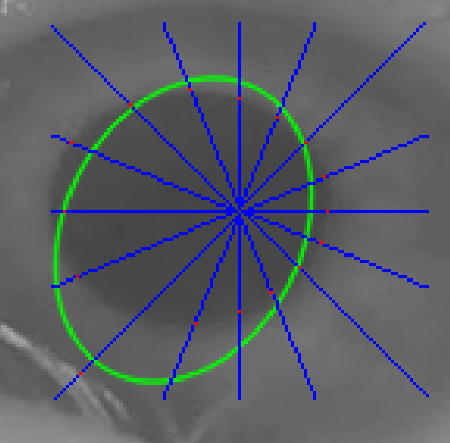
\includegraphics[width=.8\linewidth]{images/outlier_problem.png}
		\caption{Fitting of Ellipse with one outlier}
		\label{fig:oldOutlier}
	\end{subfigure}
\caption{Comparison between results with and without an outlier. It shows the big impact of an outlier on the least square fitting.}

\end{figure}

To mitigate the influence of outlier the occurrence needs to be reduced accompanied by the detection of outliers that are still detected.

\section{Angle-Validation}
\label{sec:angleValidation}
To detect outliers it is necessary to find properties that differ strongly from the other transitions. One of those properties gets visible when the angle for each transition gets calculated with the neighbouring transitions. 

In figure \ref{fig:outlierOutside} a outlier lies on the bottom left corner of the image and outside of the pupil. The angle of the outlier is very small compared to angle of the neighbouring transitions. Those on the other hand have a greater angle than the other transition points. 

When a outlier is inside the pupil then the situation is reversed as visible in figure \ref{fig:outlierInside} where the outlier has a big angle and the adjacent transitions very small angles. 

\begin{figure}[H]
\begin{subfigure}{.33\textwidth}
	\centering
	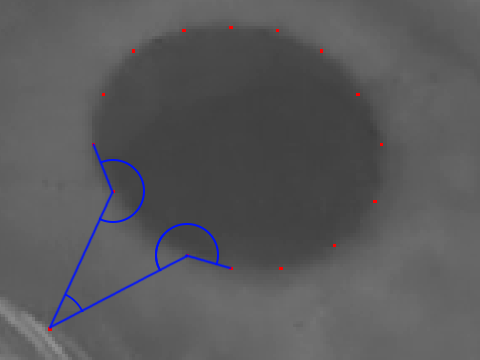
\includegraphics[width=.8\linewidth]{images/angle.png}
	\caption{Outlier outside Pupil}
	\label{fig:outlierOutside}
\end{subfigure}%
\begin{subfigure}{.33\textwidth}
	\centering
	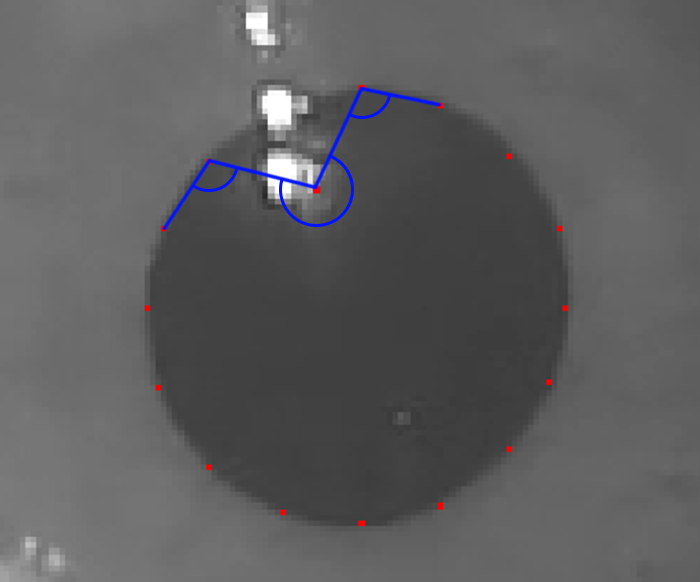
\includegraphics[width=.8\linewidth]{images/outlier_inner.png}
	\caption{Outlier inside Pupil}
	\label{fig:outlierInside}
\end{subfigure}
\begin{subfigure}{.33\textwidth}
	\centering
	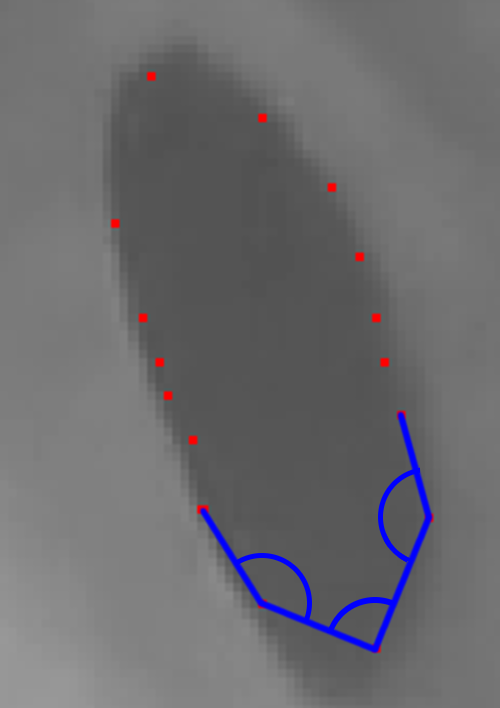
\includegraphics[width=.6\linewidth]{images/non_outlier.png}
	\caption{Accurate Transitions  with small Angles}
	\label{fig:nonOutlier}
\end{subfigure}
\caption{Angles between Transitions around Outliers}
\end{figure}

Multiple adjacent outliers differ in that it is not possible to make a clear statement what the angle will be. But the neighbours to the Outliers still have the same properties as described in the last paragraphs. For that reason an algorithm that wants to detect outliers should focus on detecting the neighbours of outliers.

In figure \ref{fig:nonOutlier} three adjacent transitions have angles that appear too small compared to its neighbours. None of them are outliers.

\subsubsection{Overview of Algorithm}
\label{sec:descriptionOfAngleValidation}

The algorithm to detect outliers based on the angles between transitions involves four steps:

\begin{enumerate}
	\item Calculate angles
	\item Find 3 adjacent angles with small differences
	\item Categorize angles
	\begin{itemize}
		\item To big
		\item To small
		\item As expected 
	\end{itemize}
	\item Determine outliers
\end{enumerate}
\subsubsection{Calculate Angles}
\label{sec:calculateAngles}
The angle between the points is calculated with the vectors that stretch from the center point to the other points. For each vector the angle between the x axis and the vector is calculated with the atan2 function. The advantage of the atan2 over the conventional arctangent function is that it takes coordinates and returns the angle for the correct quadrant. The difference of the resulting two angles is the desired angle between the points. 

When the detected transitions are close to each other, measurement uncertainty can greatly affect the angles at such points. To mitigate that effect the angle for a point is only calculated with transitions that are distant enough.
\subsubsection{Find adjacent angles with small differences}
Context is important to categorize an angle. Only angles that are as expected do not always require context. This is the case when there are three adjacent angles that fall within a narrow range of each other and create context for the neighbouring angles.

\subsubsection{Categorize Angles}
The found context leads the way to iterate over every transition and categorize the angle within the context. This is done as described in the decision making diagram in \ref{fig:decisionMaking}. Angles are classified into three groups. Angles that are as expected, too big or too small. 

\begin{figure}[H]
	\centering
	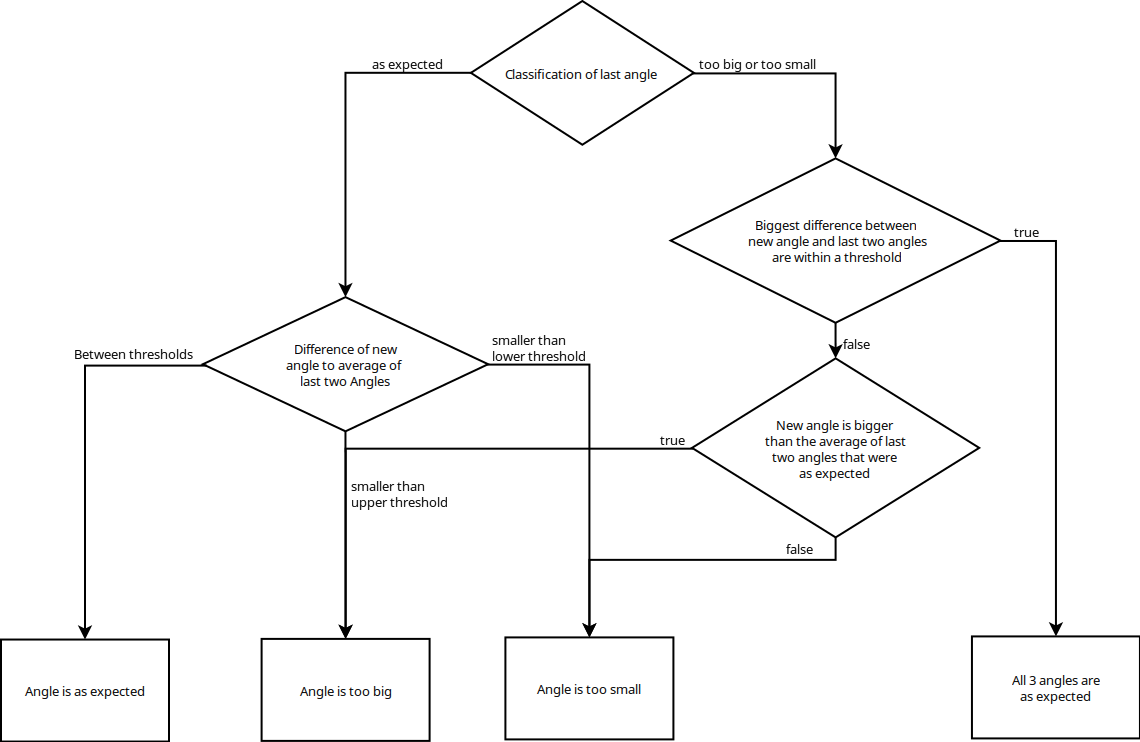
\includegraphics[width=.9\linewidth]{images/angleclassification.png}
	\caption{Decision making diagram for categorizing angles}
	\label{fig:decisionMaking}
\end{figure}
\subsubsection{Determine outliers}
As described in section \ref{sec:angleValidation} outliers are surrounded by angles that are not as expected. The categorized angles make that determination straight forward. An outlier is a transition where neither the angle before or after is categorized as expected. 
The situation described in figure \ref{fig:nonOutlier} where accurate transitions build three adjacent angles that are smaller than expected constitute an exception to this rule. This exception only occurs with adjacent small angles with neighbours that are as expected. 
\section{Colour of the Startpoint}
\label{sec:colorStartpoint}
The pupil has an uniform colour. So transitions that go from the pupil to the iris start with a colour close to the colour of the startpoint. Transitions from the iris to an eyelid on the other hand start with a colour that is brighter. This correlation can be exploited to improve the number of correctly detected transitions by dividing the score during the filter by the difference to the colour of the startpoint. To avoid a division with zero the absolute difference with an offset is used. Th offset can also be used to control the influence of this part of the algorithm.  
\section{Border Detection}
\label{sec:randdetektion}
The colours of te starburst are represented by the values between one and 255. When a point of the starburst is outside the image it is set to zero. With that it is simple to detect the border during the filter. The behaviour in this case is different depending if there was already a edge or not. If there was already an edge we would like to keep that edge otherwise the result of this ray should be discarded. 

To decide if an edge has already occurred a similar method as in section \ref{sec:colorStartpoint} is used. But instead of adjusting the score of a transitions a hard threshold is applied. 
\section{Exploit good Results}
\label{sec:goodResults}

The high framerate of the eye-capturing cameras results in small differences of the pupil position between frames. This can be used to improve the result because we already have an idea what the ellipse will look like. The startpoint can be adjusted to be the center ofthe old ellipse so the detected edges will be more equally distributed.

With the old ellipse it is also possible to calculate where a ray would transits this ellipse. This information is used to weight the score of a transition similar as the colour of the startpoint in section \ref{sec:colorStartpoint} was handled. The score is divided by the absolute distance in pixel to the old ellipse on the ray with a small offset.
\section{Fixed Threshold}
\label{sec:fixedThreshold}
This section is about a method that replaces the ray transition that uses a filter with a threshold. 

An edge is detected when the difference to the colour of the startpoint is greater than a certain threshold. 

As shown in chapter \ref{chap:results} this produces better result than the filter. Although the fixed threshold might cause problems under certain light conditions. Further analysis is needed to evaluate that risk. But even if it turns out to be a problem, there are ways to improve the idea. On such idea would be to calculate edges with multiple thresholds and use a Kalman filter to improve the result.
\section{Special Cases}
\label{sec:specialCases}
There are a number of special cases that need to be taken into account. They are likely to get forgotten but can cause major problems later on.

\begin{labeling}{\textbf{Pupil not darkest spot}}
	\item [\textbf{Closed Eyelid}] The algorithm can't produce a valid result when an eyelid is closed. Somewhere it needs to be detected when this is the case otherwise random results are produced. Without the angle validation this would be pretty straight forward as a closed eyelid would cause a bad fitting, which would cause high residuals. With the angle validation it gets a little more complex. Points that are classified as outliers are ignored. With less points it is simpler to get a good fit on random data. To minimize that risk an ellipse is only fitted when at least eight edges were not classified as outliers.
	
	There is also the option to validate a fitted ellipse later by comparing it to other fittings in the same area. 
	\item [\textbf{Pupil partly visible}] It is still possible to fit an ellipse when only a part of the pupil is visible. As described in section \ref{sec:randdetektion} the border is already detected. If the ray did not transit an edge, then the ray is ignored. The quality of the fitting will be generally lower due to the reduced number of valid edges.
	\item [\textbf{Light reflections}] Light reflections inside the pupil will cause an inner outlier. With the angle validation the edges that are detected that way should be ignored.
	
	In case the reflection is right at the startpoint everything will fail as the colour of the startpoint is assumed to be dark and similar to the rest of the pupil in sections \ref{sec:colorStartpoint} and \ref{sec:randdetektion} . The algorithm with a fixed threshold will fail when this is the case.
	
	A reflection outside the pupil will likely cause an outlier outside the pupil when measurements described in sections \ref{sec:colorStartpoint} and \ref{sec:goodResults} are not sufficient to prevent it. 
	
	Generally reflections may cause major problems and should be eliminated. By placing the infrared LEDs correctly and using glasses that filter infrared light.
	\item [\textbf{Pupil not darkest spot}] This case needs to be prevented at all cost. Otherwise the startpoint will be completely wrong and a correct fitting is not possible.
\end{labeling}

\section{Summary}
This chapter gives a overview of the existing algorithm for digitally detecting the pupil. A convenient way to visually validate the result is presented in section \ref{sec:improveTesting}. This enables a better analysis of the problems with the algorithm. The findings were applied to a variety of different methods to improve the result of the algorithm. Additionaly a different approach was proposed to detect edges with a fixed threshold. A number of special cases are discussed in section \ref{sec:specialCases}.

The validation of the algorithm is done visually. This is a good approach for a first step in improving the algorithm. Different algorithm that produce similar good results can not compared meaningful as there will be a personal bias remaining. For that reason the next chapter compares the performance of the algorithm that uses a fixed threshold and the algorithm that uses a filter to detect edges.




\chapter{Conclusion}
\label{chap:conclusions}
The realistic 3D model of the human eye and GazelleGlasses lays the foundation to test methods that calculate the gaze direction from images of the eyes. It is simple to perform additional test as no knowledge of the 3D modelling software is needed to create new test scenarios. The model is versatile as many different parameters can be configured. 

The algorithm to digitally detect the pupil is much more stable and accurate. One of the reasons for that is an ingenious method to eliminate detected edges that don't lie on the border between the pupil and the iris. Those edges would otherwise distort the result and make an accurate eye-tracking impossible.

A test with data from the model shows that a higher resolution improves the accuracy of the eye-tracking. 

%---------------------------------------------------------------------------

% Selbst�ndigkeitserkl�rung
%---------------------------------------------------------------------------
\cleardoublepage
\phantomsection 
\addcontentsline{toc}{chapter}{Declaration of authorship}
\chapter*{Declaration of primary authorship}
\label{chap:declaration_authorship}

\vspace*{10mm} 

I / We hereby confirm that I / we have written this thesis independently and without using other sources and resources than those specified in the bibliography. All text passages which were not written by me are marked as quotations and provided with the exact indication of its origin. 

\vspace{15mm}

\begin{tabbing}
xxxxxxxxxxxxxxxxxxxxxxxxxxxxxx\=xxxxxxxxxxxxxxxxxxxxxxxxxxxxxx\=xxxxxxxxxxxxxxxxxxxxxxxxxxxxxx\kill
Place, Date:		\> [Biel/Burgdorf], \versiondate \\ \\ 
Last Name/s, First Name/s:	\> [Test Peter] 	\> [M\"uster R\"os\"a] \\ \\ \\ \\ 
Signature/s:	\> ......................................\> ...................................... \\
\end{tabbing}

%---------------------------------------------------------------------------

% Glossary
%---------------------------------------------------------------------------
\cleardoublepage
\phantomsection 
\addcontentsline{toc}{chapter}{Glossay}
%\renewcommand{\glossaryname}{Glossay}
\printglossary
%---------------------------------------------------------------------------

% Bibliography
%---------------------------------------------------------------------------
\cleardoublepage
\phantomsection 
\addcontentsline{toc}{chapter}{Bibliography}
\bibliographystyle{IEEEtranS}
\bibliography{database/bibliography}{}
%---------------------------------------------------------------------------

% Listings
%---------------------------------------------------------------------------
\cleardoublepage
\phantomsection 
\addcontentsline{toc}{chapter}{List of figures}
\listoffigures
\cleardoublepage
\phantomsection 
\addcontentsline{toc}{chapter}{List fo tables}
\listoftables
%---------------------------------------------------------------------------

% Index
%---------------------------------------------------------------------------
\cleardoublepage
\phantomsection 
\addcontentsline{toc}{chapter}{Index}
\printindex
%---------------------------------------------------------------------------

% Attachment:
%---------------------------------------------------------------------------
\appendix
\settocdepth{section}
\chapter{Inserts}
\begin{enumerate}
	\item Guide to Generate an Animation
	\item Content of CD-ROM
\end{enumerate}
\chapter*{Insert 1}
\cleardoubleemptypage
\chapter*{Guide to Generate an Animation}
\label{chap:appendix_arb}
\begin{enumerate}
	\item Organise a PC, laptop or server that is powerful enough to render and runs linux.
	\item Install blender, git, ffmpeg and make on it. 
	\begin{itemize}
		\item On Ubuntu or Debian this is done with 
		
		\texttt{apt install blender make git ffmpeg}
		\item On Arch Linux this is done with 
		
		\texttt{pacman -S blender make git ffmpeg}
	\end{itemize}
	\item Clone the git repository
	
	\texttt{ git clone https://github.com/timoll/eye-generator}
	
	In case you want to contribute to the project, fork the project on github and clone your repository. Once you made meaningful changes you can push them to your repository and create a pull request.
	\item Change directory into the cloned project
	
	\texttt{cd eye-generator}
	\item There are already a few animations stored in the repository. Open a .json file for reference.
	
	\texttt{gedit animation.json}
	
	You can adjust the values manualy, write a script that generates the animation you want or modify it on \url{http://jsoneditoronline.org/} 
	\begin{labeling}{Right/Left Eye Keyframes   }
		\item [Eye Position Left/Right] Position of the Left/Right Eye in centimeters. 
		\item [Diameter] Diameter of the eye in millimetres
		\item [Last Frame] The last frame that will be rendered
		\item [Right/Left Eye Keyframes] Keyframes of the Left/Right eye. Frames in between are interpolated
		
		\begin{labeling}{Rotationnn}
			\item[Frame] When the eye has this position
			\item[Rotation] The direction the eye is looking \{-90, 0, 0\} is forward. Change x for up/down and z for left/right
		\end{labeling}
		\item [Glasses Keyframes] Keyframes for the glasses
		\begin{labeling}{Rotationnn}
			\item[Frame] When the eye has this position
			\item[Position] Position of the Glasses \{0 , 0, 0\} is a good start
			\item[Rotation] The direction the glasses is pointing \{-90, 0, 0\} is forward. 
		\end{labeling}
	\end{labeling}
	\item Save the new json file in the same folder as the rest of the project
	\item Export your file so make knows it
	
	\texttt{export ANIMATION\_JSON=myanimation.json}
	\item Create the different blend files with your animation
	
	\texttt{make}
	\item (optional) Verify that your animation is right in blender
	
	\texttt{blender leftup.blend}
	
	In the bottom left corner select "Timeline" and play the animation. You can zoom out or in by scrolling and move around by pressing the middle mouse button.
	\item Start the render, make sure this is done on the server if you have access to one. 
	
	\texttt{make render}
	It will start the render detached so you can continue to use the command line. If you want to abort the render you need to stop blender
	
	\texttt{pkill blender}
	
	Note: this will kill every instance of blender so make sure you save open blend files first.
	\item Wait, this process may take some time, especially if the pc is not that fast.
	\item Once all frames are rendered you can inspect them in their folders. The blender output is saved as log in log/renderlu.log or similar for each camera.
	
	The position and rotation of the glasses and the rotation of eyes for each frame are logged also in the log folder
	\item(optional) You might want to generate a movie files from the pictures. For the eye cameras just run the script \texttt{./genffmpeg}. It will generate video files in the folder videos.
	\item Cleaning up. Once you have saved the generated data that you need. Clean up the folder by running
	
	\texttt{make clean}
	
	To delete all the blend files that are not needed and
	
	\texttt{make clean\_render}
	
	To delete all files that where generated by the render. 

\end{enumerate}
\chapter*{Insert 2}
\cleardoubleemptypage
\chapter*{Contents of CD-ROM}
\begin{lstlisting}[style=ascii-tree]
|-- eye-generator
|-- gazelle_view
|-- gazelle_view_algorithm
|-- matlab
|-- render_results
+-- thesis_latex
\end{lstlisting}




\chapter{Additional Appendix}
\label{chap:appendix_B}

\section{Test 1}
To an English person, it will seem like simplified English, as a skeptical Cambridge friend of mine told me what Occidental is. The European languages are members of the same family. Their separate existence is a myth. For science, music, sport, etc, Europe uses the same vocabulary. The languages only differ in their grammar, their pronunciation and their most common words. Everyone realizes why a new common language would be desirable: one could refuse to pay expensive translators. To achieve this, it would be necessary to have uniform grammar, pronunciation and more common words. If several languages coalesce, the grammar of the resulting language is more simple and regular than that of the individual languages. The new common language will be more simple and regular than the existing European languages. 

\subsection{Environment}
It will be as simple as Occidental; in fact, it will be Occidental. To an English person, it will seem like simplified English, as a skeptical Cambridge friend of mine told me what Occidental is. The European languages are members of the same family. Their separate existence is a myth. For science, music, sport, etc, Europe uses the same vocabulary. The languages only differ in their grammar, their pronunciation and their most common words. Everyone realizes why a new common language would be desirable: one could refuse to pay expensive translators. To achieve this, it would be necessary to have uniform grammar, pronunciation and more common words.
\chapter{Content of CD-ROM}
\label{chap:appendix_CDROM}

Content of the enclosed CD-ROM, directory tree, etc.
%---------------------------------------------------------------------------

%---------------------------------------------------------------------------
\end{document}

